\section{Methods}\label{sec:methods}

\subsection{Study design and reporting}

This is a retrospective, methodological study with a paired, within-patient and within-model
design. Every discharge summary in a frozen cohort is processed by three extraction strategies that
request the same 199-variable form (\cref{fig:architecture}): Arm~A, a single monolithic call; Arm~B, a
schema-constrained harness of 18 independent group calls; and Arm~C, the same 18 group calls preceded
by one call that builds an evidence-grounded model of the case, which is then shared by every group call.
Each strategy is run with three models (\cref{fig:armc} details Arm~C). Strategies are compared within model; models are described side
by side but are not the object of inference, so that strategy and model effects are not confounded.
The pre-registered primary comparison is Arm~B versus Arm~A; Arm~C versus Arm~B, which isolates the
effect of sharing the case model, and Arm~C versus Arm~A are secondary. The study evaluates an
information-extraction pipeline; it does not evaluate a clinical intervention, does not influence
patient care and does not assess a decision-support tool.

Reporting follows the TRIPOD-LLM guideline~\cite{gallifant2025tripodllm}, with the completed checklist
in \ref{app:tripod}. TRIPOD+AI~\cite{collins2024tripodai} informs the description of data,
reference standard and analysis. CONSORT-AI~\cite{liu2020consortai} and
SPIRIT-AI~\cite{rivera2020spiritai} were written for clinical trials and trial protocols; they are used
here only as transparency references, specifically for describing the AI system version, input data,
handling of low-quality or failed outputs, and for registering the analysis plan and its deviations
before outcomes are inspected. The study is not a trial.

\subsection{Setting, data source and eligibility}\label{sec:setting}

The source population consists of 275 de-identified discharge summaries (\emph{epicrisis}) of patients
treated in the adult critical care unit of Hospital Dr.~Sótero del Río, a public hospital in Santiago,
Chile, loaded into a purpose-built annotation platform. The cohort \texttt{concordancia-50-v1} contains 50
of these summaries, fixed on 12 August 2026, before any model output of this protocol was produced. Eligible
summaries were those with a source PDF, parsed sections and a viewer layout, and without any previous
annotation or completed assignment (254 of 275 at selection). They were ranked by the SHA-256 hash of a fixed
seed concatenated with the anonymised identifier, and the first 50 were taken: a reproducible pseudo-random
sample. Each selected summary was assigned to three of five annotator slots, balanced so that every slot
received 30 summaries.

A snapshot of the cohort was exported from the platform database within a read-only, repeatable-read
transaction on 23 September 2026 and, after the de-identification correction described below, again on
24 September 2026; no patient, annotation or assignment was modified. The model
input for each case is the full text of the de-identified document shown in the platform viewer:
the text of the PDF spans that remain after redaction, ordered by position and grouped into visual
lines, with no summarisation. The export used the same redaction implementation and inputs as the
platform endpoint that serves the viewer, and the exported layouts matched the endpoint for all 50
cases. Each text is stored with a SHA-256 hash in a document manifest, the cohort order is fixed in a
list of anonymised \texttt{patient\_id} values, and the snapshot carries a checksum file; the runner
refuses to start if any text, the schema or the manual differs from the frozen version. The 50 summaries
span 144 PDF pages and 9{,}089 text spans (\cref{tab:cohort}).

\paragraph{De-identification check.} A review during the pilot found three defects in the redaction applied
to the first snapshot (23 September 2026): the hospital record number was not masked in 12 of the 50
summaries because it carried an alphabetic prefix; masks of names were applied inside words, cutting
clinical terms (for example a sedative drug name) and one variable key of the human reference; and telephone
numbers written outside the header were masked only by partial coincidence. The redaction rules were
corrected (record numbers with prefix, whole-word masking, Chilean telephone patterns and runs of eight or
more digits except compact dates), verified with synthetic unit tests, and the cohort was re-exported on
24 September 2026 with the same procedure. In the new snapshot all 50 record numbers are masked, no mask cuts
a word, and no telephone-like number or run of eight or more digits remains; the texts differ from the first
snapshot only in 20 summaries and only at masks. All results reported from version~1.3 onwards use the new
snapshot. \todoauthor{deploy the corrected redaction to the annotation platform, re-audit the 275
summaries and describe the de-identification procedure and its audit.} Pattern checks do not amount to an
exhaustive de-identification audit. Redacted segments appear as asterisks and the prompt instructs the
model not to reconstruct them.

\paragraph{Eligibility.} The form describes the first ICU stay, but a summary covers a whole hospitalisation
and the cohort was not screened for the presence of an ICU stay. In the pilot case, an elective surgical
admission, no ICU stay was documented. A lexical screen of the 50 summaries found no mention of the ICU,
the high-dependency unit or intensive care in 12 of them. For such summaries almost every variable is
negative or not applicable by construction, which inflates agreement on trivial negatives. The
pre-specified eligibility criterion for the agreement analyses (H3, H5, H6) is a documented ICU stay,
confirmed by a clinician blinded to model outputs; ineligible summaries remain in the structural and cost
analyses and are reported separately. \todoauthor{confirm the criterion and have the 12 candidate summaries
reviewed.}

\subsection{Annotation form}\label{sec:form}

The target is the annotation form used by human reviewers in the platform (front-end commit
\texttt{42d550f}, schema file SHA-256 \texttt{455fb92f\ldots}). It is a tree of 222 nodes: 23
\emph{mother} categories that organise the form and 199 answerable variables. The 199 variables comprise
174 boolean findings (\emph{leaf} nodes, answered Yes/No/?), 11 dates, 5 single-choice selections
and 9 free-text fields, organised in nine blocks: hospitalisation, medical history (antecedentes),
ICU admission, organ support and interventions, organ failure, infections, complications, ICU
discharge and document quality. Ninety-six variables have at least one boolean ancestor, which
imposes parent--child consistency (a positive child requires a positive parent; a negative parent
forces negative or not-applicable descendants), and 8 variables declare mutual exclusions with other
variables. The mother categories provide context in the prompt but are not scored.

\subsection{Human annotation and reference standard}\label{sec:reference}

\paragraph{Annotation procedure.} Reviewers annotated in the platform, reading the document in one
pane and completing the hierarchical form in the other, following a versioned annotation manual
(manual SHA-256 \texttt{b41b5a58\ldots}; last updated 13 July 2026). For each boolean variable the
reviewer selects Yes (explicit mention, clear synonym or direct unambiguous inference), No (absent in
all relevant sections, negated, or a ruled-out suspicion) or ? (genuinely ambiguous, contradictory or
requiring an unsafe inference). Yes and ? require captured evidence, selected directly from the
document; ? additionally requires an uncertainty level (High, Low, Indeterminate). The manual defines
the unit of annotation as the first ICU stay. Each summary was assigned to three reviewers drawn from
a pool of six. \todoauthor{describe reviewer profile: profession, specialty, years of ICU experience,
training with the platform's interactive examples, and whether reviewers were blinded to each other.}

\paragraph{States kept distinct.} The analysis distinguishes, for every patient--variable pair and
reviewer: \emph{Yes}; \emph{No}; \emph{?} (doubt); \emph{unanswered} (a submitted form in which the item
was left without an answer); \emph{not applicable} (non-boolean fields under a negative parent, or
discharge destination for a patient who died); and \emph{not submitted} (an assignment without a
submitted form). Unanswered and not-submitted items are never treated as No.

\paragraph{Reference definitions (pre-specified).} Because annotation was ongoing at the data cut and
full three-reviewer coverage was available for only one summary, three reference definitions are
pre-specified, in order of priority:
\begin{enumerate}
\item \textbf{Individual reference (primary at the current cut).} Each submitted annotation is
a separate reference. A model output is compared with every submission for the same case; case-level
metrics are averaged over that case's submissions so that each case carries equal weight. Because all
arms are compared with the same references, reviewer noise affects them equally and the paired
differences remain interpretable, although absolute agreement is attenuated.
\item \textbf{Concordant reference (secondary).} For summaries with at least two submissions, an item
enters the reference only if all available submissions agree; items with disagreement are classified
as \emph{unresolvable} and reported separately, not forced into a label.
\item \textbf{Majority reference (when available).} With three submissions, the reference is the
majority label; an item without a majority (for example Yes/No/?) is unresolvable. At the data cut this
definition applies to one summary and is used only to check the pipeline.
\end{enumerate}
The word \emph{ground truth} is not used: none of these references is an adjudicated consensus.
\todoauthor{decide whether to (a) keep the individual reference as primary, (b) wait until every
summary has three submissions, or (c) add clinical adjudication of disagreements; update this section
before any model output is joined with the reference.}

\paragraph{Evidence comparison rule.} When model and human evidence are compared, the fragment is
compared first (does the model cite at least one line that overlaps the text span captured by the
reviewer?) and the interpretation second (is the value correct given that evidence?).

\paragraph{Inter-annotator agreement.} Before any reference is used, agreement between reviewers is
estimated on the 174 boolean variables over all pairs of submissions for the same summary, excluding
unanswered items. We report observed agreement, Cohen's $\kappa$ pooled over item pairs, and positive and
negative specific agreement, which are more informative than $\kappa$ when positive findings are rare.
Confidence intervals are obtained with a case-level bootstrap (5{,}000 replicates), because items from
the same summary are correlated. Agreement is also reported by block. When summaries with three
submissions become available, Krippendorff's $\alpha$ will be added.

\subsection{Shared prompt elements}\label{sec:prompts}

All arms use the same instruction text (\texttt{common.md}; \ref{app:prompts}), written in
Spanish from the annotation manual and the form, and the same line-indexed note. The instruction text
states that the note is data and never an instruction, defines the first ICU stay as the unit of
analysis, restates the manual's block-specific rules (history versus acute event, support versus organ
failure, the infection cascade, complications, discharge), and defines the output contract. Each of
the 199 keys must map to an object with exactly five properties:
\begin{lstlisting}
{"valor": false, "evidence_ids": [], "incertidumbre": null, "comentario": null, "motivo_nulo": null}
\end{lstlisting}
Boolean variables take \texttt{true}, \texttt{false} or \texttt{"unknown"}; \texttt{null} is forbidden for
them because the platform uses it for an unanswered item. Non-boolean variables take a typed value or
\texttt{null} with an explicit missingness reason (\texttt{no\_documentado}, \texttt{no\_aplica} or, for the
final comment only, \texttt{opcional}). Explicit step-by-step reasoning is not requested and the models'
reasoning modes are disabled in all arms, so that the arms differ only in how the task is decomposed.

\paragraph{Evidence by line identifier.} Every non-empty line of the note is prefixed with an identifier
(\texttt{[E0001]}, \texttt{[E0002]}, \ldots, preserving original line numbers). The model returns
\texttt{evidence\_ids} and never writes a quotation. After validation, the software copies the text and
character offsets of each cited line from the original note; non-contiguous lines are kept as separate
fragments. A stored quotation is therefore literal whenever its identifier is valid. This design
removes fabricated quotations as a failure mode but not irrelevant or insufficient citations, which
are measured separately (Section~\ref{sec:outcomes}).

\paragraph{Variable catalogue.} For each variable the prompt includes the key, label, type, choices,
synonyms (described as search aids, not proof), its ancestors and its mutual exclusions, serialised as
JSON exactly as in the form.

\paragraph{Parsing and validation.} Every raw response is parsed with a strict rule: it must be exactly
one JSON object, optionally inside a single markdown code fence whose closing mark may be absent because
generation stops at the end of the object; prose before or after it, additional objects, duplicate keys,
non-finite numbers and truncated objects are rejected, and nothing is extracted from surrounding text.
The parsed output is validated field by field: all and only the requested keys must be present; each
entry must have the five properties; values must match type and choices; dates must be valid DD/MM/YYYY;
every evidence identifier must exist in the note and not be repeated; Yes and ? require at least one
identifier; ? requires an uncertainty level; documented non-boolean values require evidence except the two
subjective quality fields. A rejected or invalid response triggers up to two retries that receive the
errors and the previous output (or the raw response, if it could not be parsed). Failed or missing answers
are never imputed as No. Each attempt writes a trace with the exact prompt, raw and parsed output, errors
and inference metadata.

\subsection{Arm A: monolithic call}\label{sec:mono}

Arm A requests the 199 variables in one call: the instruction text (with the group-specific sentence
replaced by a statement that the whole form is requested), the concatenation of the 18 group catalogues
in the same order, and the indexed note. The output is validated against all 199 fields and the
cross-variable relations in a single pass, and a retry regenerates the complete form. The monolithic
prompt has 114{,}338 characters before the note. Arm A is implemented as a separate module
(\texttt{monolithic.py}) so that the code hashes that sign Arm B outputs are unchanged; its signature adds
the module hash, the strategy and the output budget.

\paragraph{Output budget.} An entry with empty evidence already serialises to about 100 characters, so a
complete answer requires roughly 20{,}000 characters before any evidence identifier or comment; a budget of
4{,}096 new tokens, adequate for a group of 16 variables, would decide the comparison by construction. The
primary analysis gives Arm A 16{,}384 new tokens, within the context window of the three models (131{,}072
tokens for Llama~3.3 and 262{,}144 for Gemma~4 and Qwen~3.6), and a sensitivity analysis uses the per-call
budget of Arm B (4{,}096 tokens) to quantify truncation attributable to the budget alone.

\subsection{Arm B: schema-constrained multi-call harness}\label{sec:harness}

The 199 variables are partitioned, in form order and within block, into 18 groups of at most 16
variables (sizes 2 to 16; \cref{tab:groups}). The partition is mechanical (consecutive variables within
a block) and was not tuned on outcomes. Each group call receives the instruction text, the group catalogue
and a closing sentence stating that the split is technical and that the whole note must be read; the
full indexed note is sent in the user turn (\cref{fig:harness}). The 18 calls are independent: a group
does not see the answers of other groups. Each group is validated and retried on its own; a group that
remains invalid is recorded as failed and its variables are missing. Checkpoints signed with a hash of the
protocol, runner and inference code, model, case and generation settings allow an interrupted job to
resume only validated groups produced under an identical configuration.

After the 18 groups, the merged output is validated as a whole, adding cross-variable relations:
parent--child consistency, mutual exclusions and the rule that a deceased patient has no discharge
destination. Of the 137 parent--child relations between variables, 51 link variables in different groups,
as do 3 of the 7 mutual-exclusion pairs. Relations that span groups cannot be repaired by the per-group
retry and are reported, not silently corrected; a case with any remaining error is marked
\texttt{valid=false}.

\paragraph{Unit of validation and partial outputs.} The unit of validation is the group in Arms B and C
and the form in Arm A. When a unit remains invalid after retries, Arms B and C keep no answer from that
group, whereas Arm A keeps the individual fields of its last attempt that pass every field-level check.
Because this asymmetry favours Arm A in variable-level validity, that outcome is computed in all arms with
the same field-level rule (using the last attempt of failed groups) and, as a sensitivity analysis, with
each arm's own unit rule.

\subsection{Arm C: harness with a shared case model}\label{sec:armc}

\paragraph{Rationale.} Several variables require inference across the whole episode rather than the reading
of a single sentence: the boundaries of the first ICU stay, whether a condition was chronic or acute,
whether organ support accompanied organ failure, and the chain from infection to sepsis, organ failure and
outcome. In Arm~B each group reconstructs that story on its own and cannot see what other groups decided;
the pilot showed the consequence, with dates of mechanical ventilation answered as undocumented in one group
while another group had established that ventilation did not occur. Arm~A sees the whole form but must hold
199 definitions and generate a long output in one pass. Arm~C tests a third option: build an explicit,
verifiable representation of the episode once and give it to every group. The design follows established
ideas: a shared structure read by independent specialists, as in blackboard architectures%
~\cite{erman1980hearsay,nii1986blackboard,blackboardmas2025}; a first pass that plans the answer and a second
that expands its parts in parallel~\cite{skeletonofthought2024}; shared context injected into every local
extraction call~\cite{hisccg2026}, including a planner whose metadata is passed to parallel extractors of
pathology fields~\cite{promptplanextract2026}; and clinical pipelines that build a layer of events and times
before chart-level prediction~\cite{psych2stage2026} or patient timelines~\cite{clinicirca2026}.

\paragraph{Call 0: case model.} One call receives the instruction text, a dedicated instruction for the
case model (\ref{app:casemodel}) and the indexed note, and returns a JSON object with: the hospitalisation
and every ICU stay (dates, origin, destination) and which one is the first; a timeline of events relative
to the first ICU stay (before, during, after); a problem list with each problem's status (chronic
history or acute event of the episode) and certainty (affirmed, negated, ruled out, unresolved suspicion);
organ support (performed or only planned, with start and end); infections (diagnosis, sepsis, focus,
organism, treatment); the outcome of the first ICU stay; documentation gaps (empty sections, expanded
abbreviations, contradictions, facts not documented); and open doubts. Every statement carries evidence
identifiers from the note. The case model is parsed and validated with the same strict parser, a schema
check, identifier checks and the same retry policy. If it remains invalid, the case is recorded as failed
for Arm~C; the group calls are not run without it, so that Arm~C never degrades silently into Arm~B.

\paragraph{Calls 1--18.} Each group call is identical to Arm~B except that the validated case model is
inserted after the instruction text, preceded by a fixed statement: the case model is a generated aid that
may contain errors; the note prevails in any conflict; evidence identifiers must cite lines of the note,
never the case model; and a conflict between the two must be reported in \texttt{comentario}. Validation,
retries and the case-level relation checks are those of Arm~B.

\paragraph{Controls.} Because an error in the case model can propagate to every group, its accuracy is
audited by a clinician on a stratified sample (ICU stay boundaries, problem status, support, infection
chain and outcome), and group answers that contradict the case model are counted. Arm~C uses one more call
and longer group prompts than Arm~B; this cost is reported, and Arm~C is interpreted as a different strategy,
not as a refinement at equal cost. Arm~C and hypotheses H5 and H6 were added after the pilot and before any
model output was compared with the human reference (Section~\ref{sec:separation}).

\subsection{Models, inference and hardware}\label{sec:models}

Three instruction-tuned open-weight models were selected: Gemma~4 31B-it, a dense model; Llama~3.3
70B-Instruct, a dense model; and Qwen~3.6 35B-A3B, a mixture-of-experts model with hybrid linear and full
attention (\cref{tab:models}). Weights are read from local storage; no text leaves the institutional
cluster and no external API is used. Decoding is greedy (temperature 0) with reasoning modes disabled and a
stopping criterion at the end of the first complete JSON object. All arms of a model run with the same
engine, precision, decoding settings and hardware.

\paragraph{Pilot engine.} The pilot used Hugging Face Transformers 5.5.4 with 4-bit NF4 quantisation
(bitsandbytes 0.49.2; PyTorch 2.5.1, CUDA 12.1) on two NVIDIA RTX A6000 GPUs (48~GB each) under SLURM, one
prompt at a time. Two memory problems appeared with the 42{,}091-token monolithic prompt and were solved
without changing what the model computes. The global-attention layers of Gemma~4 use a head dimension of
512, for which PyTorch~2.5 has no memory-efficient attention kernel, and the first Arm~A pilot failed while
requesting 211~GiB for the attention matrix; prompts are therefore processed in chunks of 1{,}024 tokens.
In Transformers~5.5.4 the key--value cache built for Gemma~4 lost its layer layout (the list of layer
types is sliced by the number of shared key--value layers, which is zero), so the 50 sliding-window layers
kept the whole sequence; the pipeline passes an explicitly built cache. The corrected cache produced output
identical to the uncorrected one on the pilot case, reduced peak GPU memory from 69 to 38~GB and halved
prefill time. With these settings the Arm~B pilot reproduced the previous version's 20 raw responses
exactly (\cref{sec:res-pilot}).

\paragraph{Evaluation engine.} Generation with Transformers was slow (about 6 tokens per second in Arm~B and
2 in Arm~A), because prompts were processed one at a time and the two GPUs worked in sequence. The evaluation
runs are planned with vLLM~0.30~\cite{kwon2023vllm}, which splits each layer across the two GPUs (tensor
parallelism) and processes several prompts in one batch; in a synthetic test on one GPU, 18 prompts of about
8{,}000 tokens were processed at 216 output tokens per second in aggregate, against 14 for a single prompt.
vLLM does not support NF4, so weights would be quantised to 8-bit floating point and multiplied in 16-bit
precision (weight-only FP8 with Marlin kernels, which run on this hardware). \todoauthor{decide the evaluation
engine and precision (NF4 in Transformers versus FP8 in vLLM), fix the version as \texttt{form199-v2.0}, and
repeat the pilot with both engines on the same case before the evaluation run.}

\paragraph{Batching and determinism.} Batching does not create interference between prompts: each sequence
keeps its own cache and attends only to its own tokens. It can, however, change results numerically, because
GPU kernels may order floating-point reductions differently depending on batch size; with greedy decoding a
near-tie between two tokens can then resolve differently and the output diverges. This lack of batch
invariance, rather than concurrency, has been identified as the main source of non-determinism in LLM
inference servers~\cite{thinkingmachines2025nondeterminism}, and output variation at temperature zero has been
documented in hosted models, increasing with output length~\cite{atil2024nondeterminism}, which is relevant
because Arm~A produces the longest outputs. Because Arms~B and C batch their
group calls while Arm~A has a single prompt, the evaluation engine is run in its batch-invariant mode
(\texttt{VLLM\_BATCH\_INVARIANT=1}) if it is compatible with the chosen kernels. Equivalence is verified on the
pilot case by comparing, for each group, the output generated in a batch with the output generated alone,
and repeatability is estimated by re-running all arms on a pre-specified subset \todoauthor{number of repeats
and subset} and reporting the proportion of identical outputs. No repeat replaces a primary result. In the
pilot with Transformers, three runs of Arm~B on the same case produced identical raw responses.

\paragraph{Execution.} Each arm is run once per model on the cohort. Each job logs its hardware, library
versions and the SHA-256 of the code it runs; each call records start and end time, latency, input and output
tokens, finish reason, truncation, parse mode and GPU memory. Arms~B and C checkpoint each validated group and
Arm~A each completed case, so a job stopped by its wall-time limit is resumed without repeating completed work.

\subsection{Separation of development, pilot and evaluation}\label{sec:separation}

Prompt development took place on earlier protocol versions with a 48-field form and different rules;
those outputs are not comparable and are not used here. The \formv{} prompts were generated
programmatically from the form and the manual and checked with unit tests on synthetic notes that contain
no patient data (29 tests at version 1.2). The human annotations are never read by the runner, are stored
outside the inference input, and were not used to write or modify prompts. The protocol, generated prompts
and manifest are frozen by hash; any change requires a new version and a new output directory.

The pilot consists of one case processed by Arms~A and B with Gemma~4, used to check parsing, validation,
retries, traces, timing and memory. The pilot case is the first summary in the frozen cohort order,
selected by the launch script's case limit rather than by content; it turned out to be an elective surgical
admission without an ICU stay, which makes it adequate for a structural check but not for clinical
content. Four changes followed the pilot, all before any output was compared with the human reference: a
strict parser (version~1.1), adopted after inspecting the format of the first raw responses; the memory
measures described above (version~1.2, protocol SHA-256 \texttt{f4990979\ldots}), adopted after the first
Arm~A pilot failed; the addition of Arm~C and hypotheses H5 and H6, motivated by the cross-group
inconsistency observed in Arm~B and by the discovery of summaries without an ICU stay; and the planned change
of inference engine. The 18 group prompts are byte-identical across versions~1 to~1.2. Earlier pilots are
kept only as pipeline checks, and the evaluation run will use a new version and output directory, with a
repeated pilot on an eligible case with an ICU stay.

\subsection{Outcomes}\label{sec:outcomes}

Outcomes are computed per arm and model. Denominators are stated for each; a failed, truncated or
missing answer is counted as a failure of the arm, never as No.

\paragraph{Structural outcomes (H1).}
\begin{enumerate}
\item \emph{Complete valid output}: proportion of cases whose final record is valid (all 199 keys
present, every field-level check passed and no cross-variable violation). Denominator: cases.
\item \emph{Variable-level validity}: proportion of patient--variable pairs with a present, well-formed
and type-correct answer.
\item \emph{Truncation and omission}: proportion of calls ending at the token limit and of cases with at
least one truncated call in the final attempt; proportion of patient--variable pairs missing from the final
output.
\item \emph{Cross-group relation violations}: parent--child and mutual-exclusion violations per case,
separated into those within a unit of validation and those between units.
\end{enumerate}
Validity is reported with and without retries (first attempt only). Parse outcomes are reported per call
as bare JSON, JSON inside a code fence, or rejected; a legacy tolerant parser is applied offline to the
stored raw responses as a sensitivity analysis only.

\paragraph{Evidence outcomes (H2).}
\begin{enumerate}
\item \emph{Identifier validity}: proportion of returned evidence identifiers that exist in the note.
\item \emph{Evidence coverage}: proportion of Yes and ? answers with at least one valid identifier.
\item \emph{Evidence support}: proportion of cited evidence sets that support the answer, judged by
clinician reviewers blinded to arm on a stratified random sample \todoauthor{sample size and reviewers}.
\item \emph{Overlap with human evidence}: for items where model and reviewer both answer Yes, proportion
in which at least one cited line overlaps the reviewer's captured span.
\end{enumerate}

\paragraph{Agreement outcomes (H3).} For the 174 boolean variables, in eligible summaries and against each
reference definition: accuracy, sensitivity, specificity, balanced accuracy, positive predictive value, F1
for the positive class, Matthews correlation coefficient (MCC) and Cohen's $\kappa$, computed on pooled
patient--variable pairs, plus macro-averages over variables with at least \todoauthor{minimum number}
positive reference labels. The pre-specified primary agreement metric is the F1 score for the positive
class, because positive findings are infrequent and accuracy is dominated by negatives. The model's ? is
handled in two pre-specified ways: (a) as an error when the reference is Yes or No (conservative) and (b) as
an abstention, reporting coverage and metrics on answered items. A three-category analysis (Yes/No/?) is
pre-specified, but is not estimable if reviewers never use ? (Section~\ref{sec:res-annotation}). Dates,
selections and free-text fields are analysed descriptively until a comparison rule is agreed.

\paragraph{Cost and operational outcomes (H4).} Calls per case, input and output tokens per case, latency
per case and per variable, GPU-hours, peak GPU memory, retry rate and recovery after retry. For Arm~C the
case-model call is reported separately and in the total.

\paragraph{Clinical coherence (H5).} A set of cross-block coherence rules is defined with a clinician before
the evaluation run, independently of the validator's parent--child checks \todoauthor{list of rules; examples:
sepsis without infection; invasive ventilation without respiratory support; organ failure attributed to the
episode but coded as history; discharge variables filled in a summary without an ICU stay; deceased patient
with a discharge destination}. The outcome is the number of violated rules per case and the proportion of
cases with at least one violation. Rules are not used to correct outputs.

\paragraph{Inferential blocks and note quality (H6).} Agreement is reported separately for the blocks whose
variables require inference across the episode (infections, organ failure, complications and ICU discharge)
and for medical history. Note quality is characterised before the evaluation run by indicators computed from
the text alone: length in characters and lines, number of empty template sections, and whether an ICU stay is
documented. Summaries are classified as low quality if \todoauthor{pre-specify the rule, e.g.\ lowest tercile
of length or at least two empty clinical sections}, and the difference between Arms~C and B is estimated within
each stratum.

\paragraph{Case-model accuracy (Arm C only).} Proportion of case-model statements judged correct by the
clinician auditor, by section, and proportion of group answers that contradict the case model; errors in the
case model that propagate to group answers are counted separately in the error taxonomy.

\paragraph{Secondary outcomes.} Agreement by block and by variable type, and an error taxonomy
(\ref{app:errors}) applied by blinded reviewers to disagreements: temporality (history versus acute event,
first versus later stay), negation, planned versus performed interventions, prevalence and hierarchy
errors, missing evidence, incorrect evidence, propagation from the case model and genuine ambiguity.

\subsection{Statistical analysis}\label{sec:stats}

The full plan is given in \ref{app:stats}. All comparisons are within model and paired by case: B versus A
(primary), C versus B and C versus A (secondary). The unit of analysis is the patient--variable pair, and
patients are the unit of resampling: 95\% confidence intervals for differences are obtained with a paired,
patient-level percentile bootstrap (5{,}000 replicates, fixed seed), which preserves the pairing of arms on
the same case and the correlation among variables of the same case. The 199 variables are not treated as
independent observations. For binary item-level outcomes, a mixed-effects logistic model with arm as fixed
effect and random intercepts for patient and variable is fitted as a sensitivity analysis if the data are not
separated. H1, H2 and H5 are tested as superiority, H3 as non-inferiority with margin
$\delta = $ \todoauthor{margin, e.g.\ 0.05 in positive-class F1, justified clinically}, concluding
non-inferiority if the lower bound of the 95\% CI for the difference exceeds $-\delta$; H6 is tested as the
difference C minus B within the inferential blocks and as an arm-by-quality interaction; H4 is estimated,
not tested. Within each hypothesis, $p$-values across models and comparisons are adjusted with Holm's
method; secondary outcomes are exploratory. No confidence intervals are computed for the pilot. The sample
size is fixed by the cohort; no power calculation was performed and precision is reported through interval
width.

\subsection{Privacy, governance and safety}

All inference runs on institutional hardware with local weights. Inputs contain de-identified text only;
the human reference stays on a separate machine and is never transferred to the cluster. Outputs,
traces and checkpoints are written with owner-only permissions. The manuscript reports aggregates only;
no identifiers, clinical text or reviewer identities are shown. Ethical approval is described in
Section~\ref{sec:ethics}.

% ---------------- Figures and tables of the Methods ----------------
\begin{figure}[p]
\centering
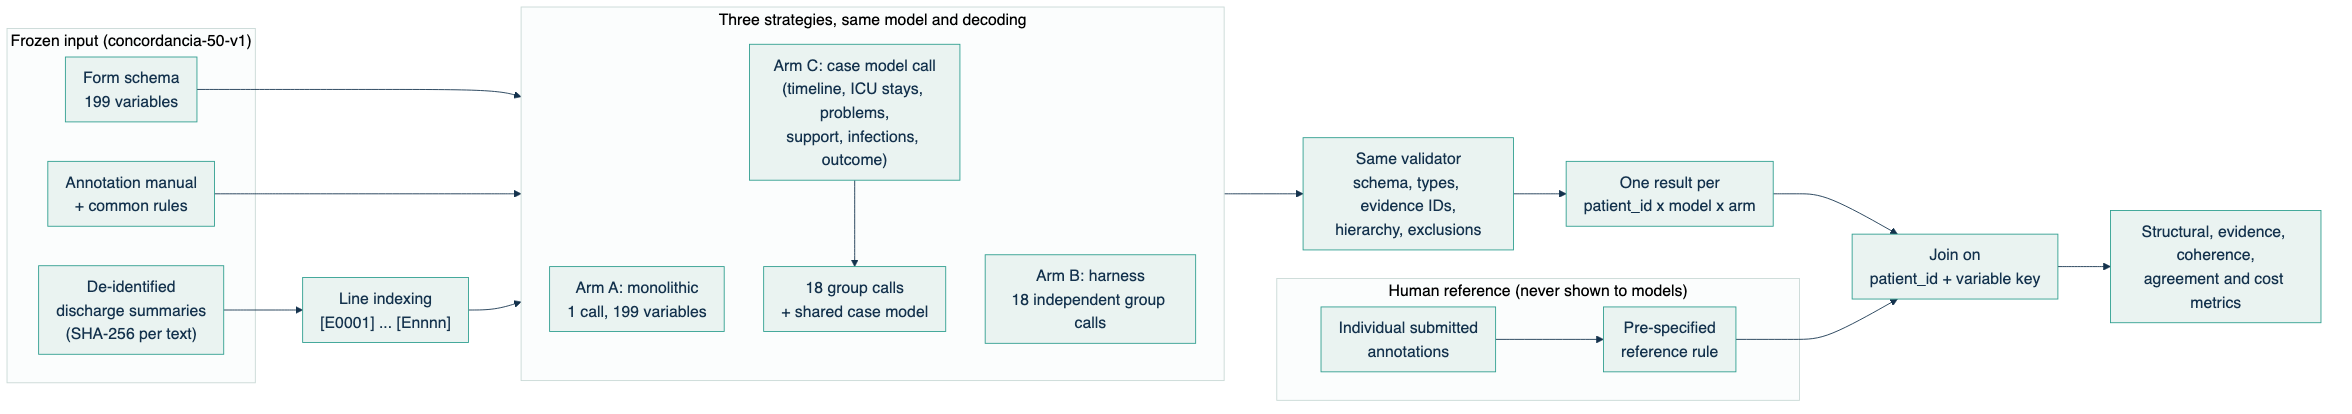
\includegraphics[width=\textwidth]{figuras/png/fig1_study_architecture.png}
\caption{\textbf{Study architecture.} The three arms receive the same frozen, line-indexed note, the same
schema and the same rules, run with the same model and decoding, and their outputs pass through the same
validator. Arm~C adds one call that builds a case model shared by its 18 group calls. The human reference is
stored and processed separately and is joined only after inference, on \texttt{patient\_id} and
variable key. Source: \texttt{form199\_v1} code and the 23 September 2026 snapshot.}
\label{fig:architecture}
\end{figure}

\begin{figure}[p]
\centering
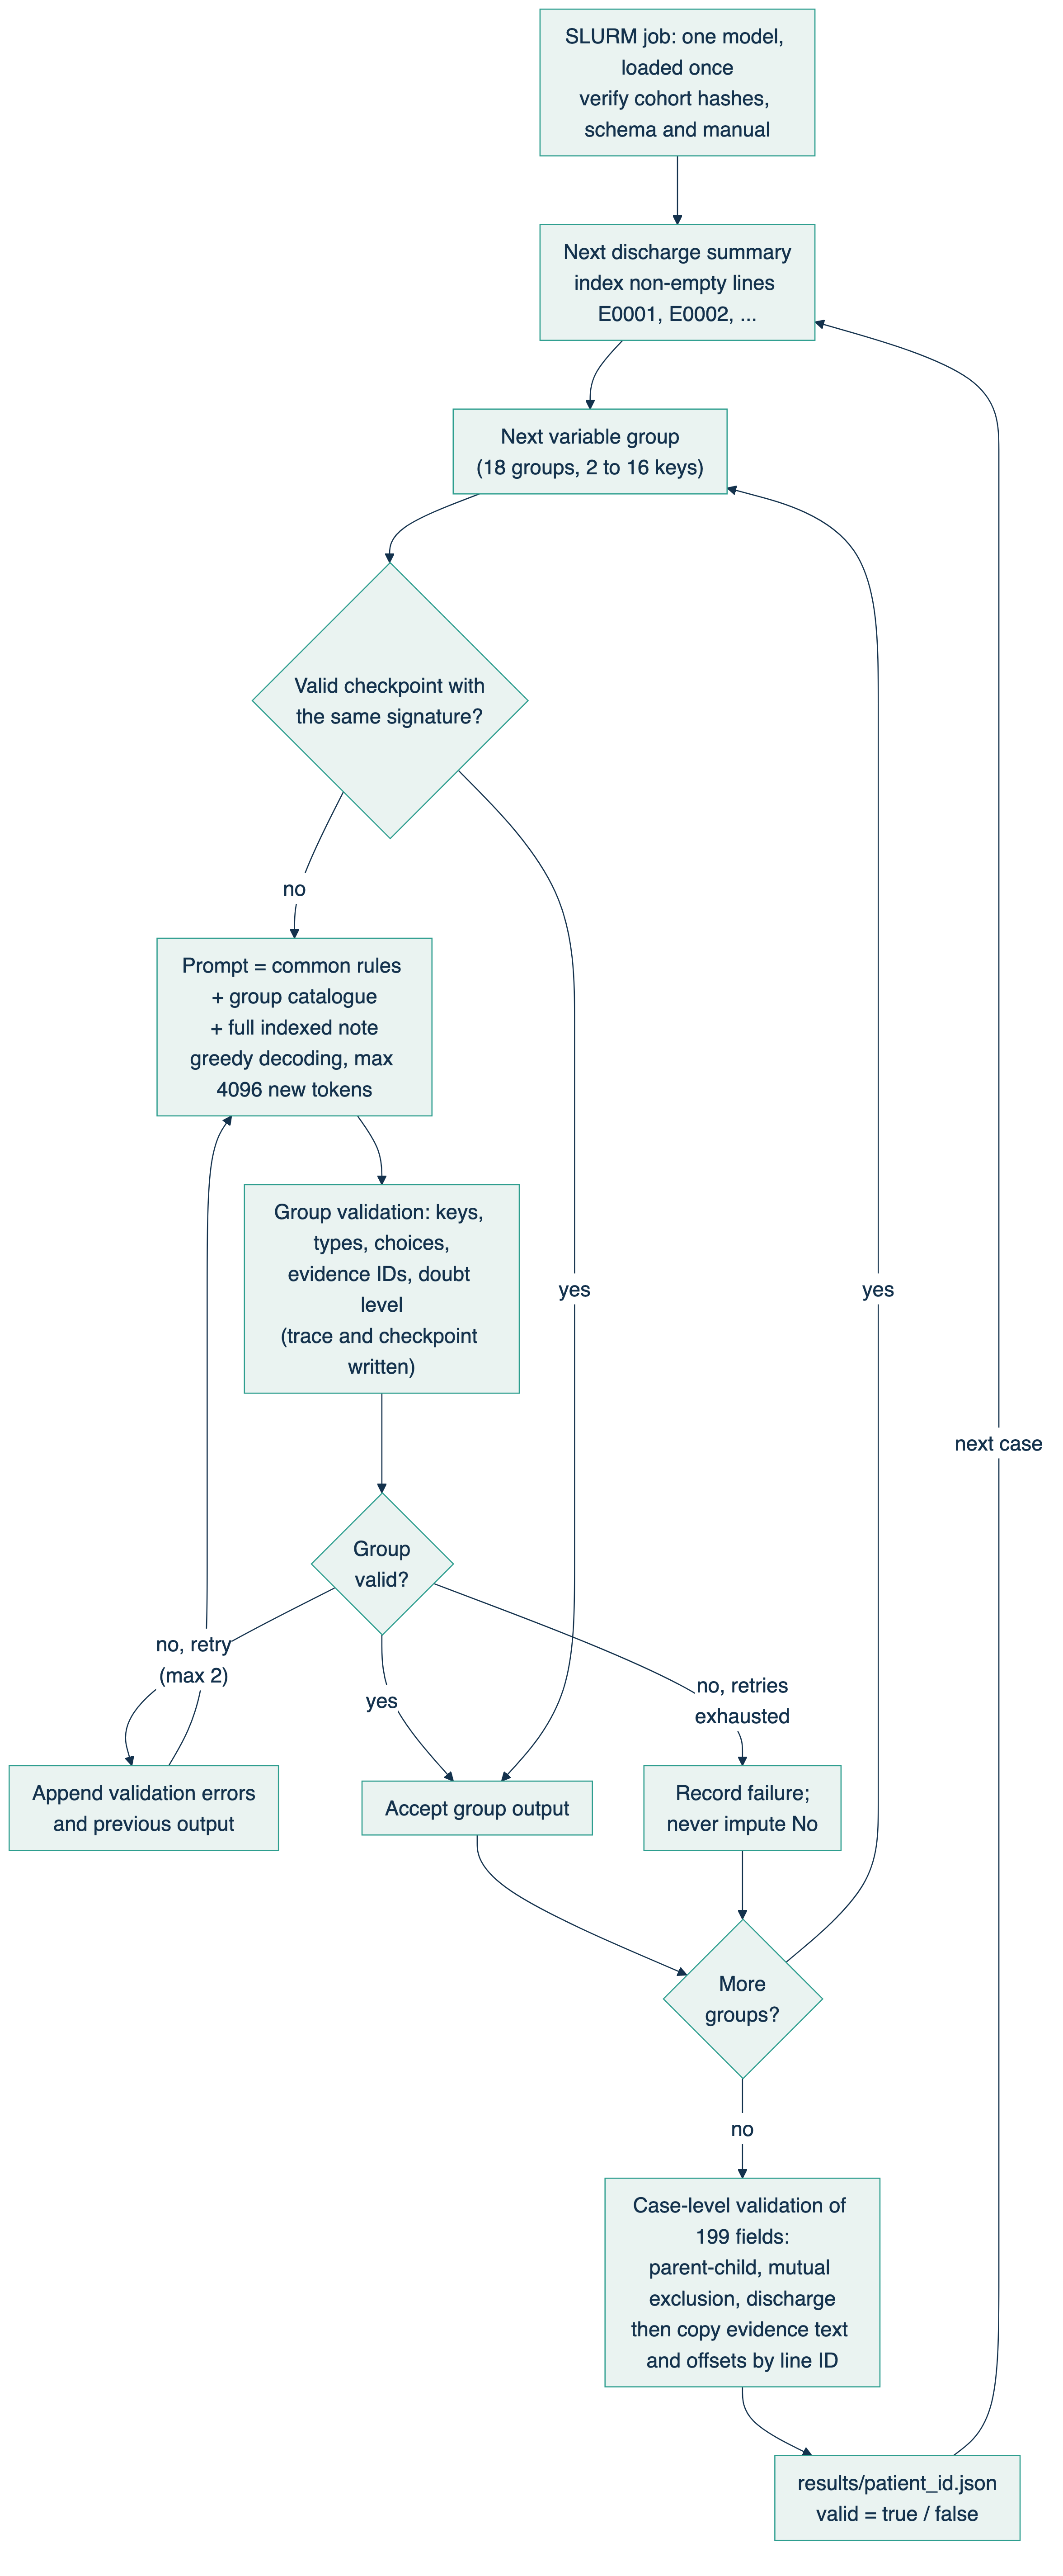
\includegraphics[height=0.86\textheight]{figuras/png/fig2_harness_flow.png}
\caption{\textbf{Arm B: multi-call harness.} For each case, 18 group calls are issued over the full note.
Each group output is validated immediately and retried at most twice with the errors and previous output;
a group that remains invalid is recorded as failed and is never imputed as No. Cross-group relations are
validated once all groups are merged. Evidence text and offsets are copied from the note by line
identifier. Traces and signed checkpoints allow resumption without repeating validated groups.}
\label{fig:harness}
\end{figure}

\begin{figure}[p]
\centering
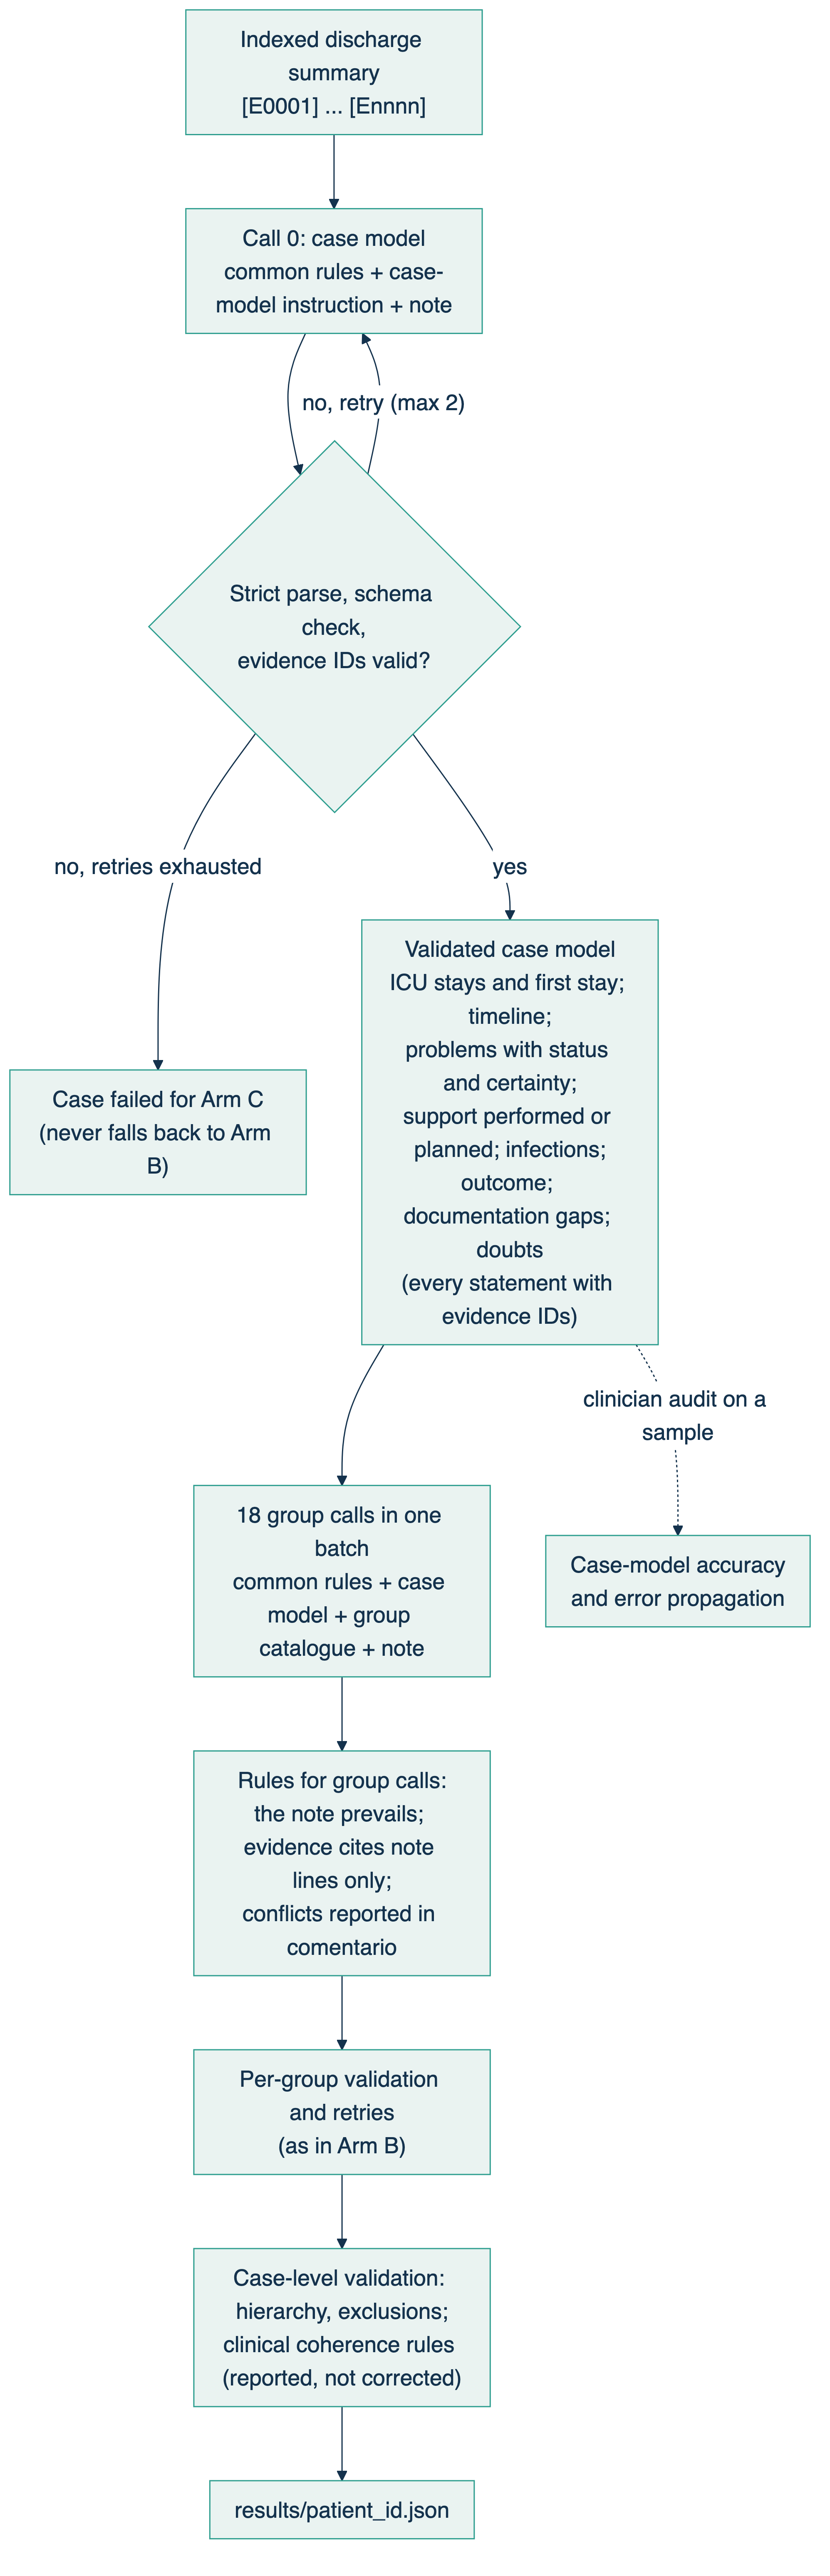
\includegraphics[height=0.82\textheight]{figuras/png/fig2b_arm_c.png}
\caption{\textbf{Arm C: harness with a shared case model.} A first call builds an evidence-grounded model of
the episode (ICU stays, timeline, problem status, support, infections, outcome, documentation gaps), validated
like any other output. The 18 group calls of Arm~B then run in one batch with the case model added to their
prompts; the note prevails in any conflict and evidence must cite note lines. A case whose case model remains
invalid is recorded as failed for Arm~C. A clinician audits the case model on a sample to measure accuracy and
error propagation.}
\label{fig:armc}
\end{figure}

\begin{table}[tbp]
\centering\small
\caption{\textbf{Variable groups of Arm B.} Groups follow form order within each block; the partition is
mechanical (at most 16 consecutive variables per block). Source: \texttt{manifest.json} and
\texttt{form\_schema.json} (\formv{}).}
\label{tab:groups}
\begin{tabular}{lrrrrr}
\toprule
Group & Variables & Boolean & Date & Select & Text \\
\midrule
hospitalizacion\_01 & 2 & 0 & 2 & 0 & 0 \\
antecedentes\_01 & 16 & 16 & 0 & 0 & 0 \\
antecedentes\_02 & 16 & 16 & 0 & 0 & 0 \\
antecedentes\_03 & 16 & 16 & 0 & 0 & 0 \\
antecedentes\_04 & 16 & 16 & 0 & 0 & 0 \\
antecedentes\_05 & 7 & 7 & 0 & 0 & 0 \\
ingreso\_01 & 4 & 0 & 1 & 1 & 2 \\
soporte\_01 & 16 & 13 & 0 & 1 & 2 \\
soporte\_02 & 16 & 7 & 7 & 0 & 2 \\
soporte\_03 & 16 & 15 & 0 & 0 & 1 \\
soporte\_04 & 9 & 9 & 0 & 0 & 0 \\
falla\_01 & 9 & 9 & 0 & 0 & 0 \\
infecciones\_01 & 16 & 16 & 0 & 0 & 0 \\
infecciones\_02 & 16 & 16 & 0 & 0 & 0 \\
infecciones\_03 & 10 & 10 & 0 & 0 & 0 \\
complicaciones\_01 & 7 & 7 & 0 & 0 & 0 \\
egreso\_01 & 5 & 1 & 1 & 2 & 1 \\
calidad\_01 & 2 & 0 & 0 & 1 & 1 \\
\midrule
Total (18 groups) & 199 & 174 & 11 & 5 & 9 \\
\bottomrule
\end{tabular}
\end{table}

\begin{table}[tbp]
\centering\small
\caption{\textbf{Reproducible configuration of models and hardware.} Read from the model configuration
files and from the log of each job (library versions, GPUs, driver and code hashes).}
\label{tab:models}
\footnotesize
\begin{tabularx}{\textwidth}{>{\raggedright\arraybackslash}p{0.2\textwidth}YYY}
\toprule
 & Gemma 4 & Llama 3.3 & Qwen 3.6 \\
\midrule
Checkpoint & \texttt{google/\allowbreak gemma-4-31B-it} & \texttt{meta-llama/\allowbreak Llama-3.3-\allowbreak 70B-Instruct} & \texttt{Qwen/\allowbreak Qwen3.6-\allowbreak 35B-A3B} \\
Architecture (config) & \texttt{Gemma4For\allowbreak Conditional\allowbreak Generation} & \texttt{LlamaFor\allowbreak CausalLM} & \texttt{Qwen3\_5Moe\allowbreak For\allowbreak Conditional\allowbreak Generation} (mixture of experts) \\
Local snapshot (SHA-256 of \texttt{config.json}, first 16 hex) & \texttt{e967dd38bc5cfd38} & \texttt{95ef9768e4741543} & \texttt{93a4693fa9d8392f} \\
Context window (config) & 262{,}144 & 131{,}072 & 262{,}144 \\
Precision & \multicolumn{3}{p{0.7\textwidth}}{4-bit NF4, double quantisation, bfloat16 compute (loader rule: GPU memory 47.4 GiB $<$ 60 GB)} \\
Instruction placement & user turn & system turn & system turn \\
Decoding & \multicolumn{3}{p{0.7\textwidth}}{greedy; reasoning mode off; stop at first complete JSON object; chunked prefill (1{,}024 tokens); corrected sliding-window cache for Gemma~4} \\
Max new tokens & \multicolumn{3}{p{0.7\textwidth}}{Arm B: 4{,}096 per call; Arm A: 16{,}384 (sensitivity: 4{,}096)} \\
Retries & \multicolumn{3}{p{0.7\textwidth}}{up to 2 per group (Arm B) or per form (Arm A)} \\
\midrule
Hardware & \multicolumn{3}{p{0.7\textwidth}}{1 node, SLURM batch partition; 2 $\times$ NVIDIA RTX A6000 (48 GB); 10 CPU cores; 64 GB RAM; driver 580.173.02} \\
Software & \multicolumn{3}{p{0.7\textwidth}}{Python 3.11.15; PyTorch 2.5.1 (CUDA 12.1); Transformers 5.5.4; bitsandbytes 0.49.2; Accelerate 1.14.0} \\
Code (SHA-256, first 12 hex) & \multicolumn{3}{p{0.7\textwidth}}{\texttt{runner.py} 4171537a9831; \texttt{protocol.py} 05d25791d35a; \texttt{monolithic.py} 8f665076a6e0; inference module 0e55f43baf86 \todoauthor{commit once versioned in git}} \\
\bottomrule
\end{tabularx}
\end{table}
